\documentclass[a4paper,12pt]{report}

\usepackage{alltt, fancyvrb, url}
\usepackage{graphicx}
\usepackage{subfigure}
\usepackage{wrapfig}
\usepackage{algorithmic}
\usepackage[utf8]{inputenc}
\usepackage{fontenc}
\usepackage{amsmath,stmaryrd,mathtools,algorithm}
\usepackage{amssymb}
\usepackage{float}
\usepackage{hyperref}

% Remove option to use English naming
\usepackage[italian]{cleveref}

% Questo commentalo se vuoi scrivere in inglese.
\usepackage[italian]{babel}

\graphicspath{ {./images/} }

\begin{document}
	\title{\Huge \textbf{Quoridor2D} \\ \vspace{0.4cm} \large Relazione progetto OOP}
	\author{Becci Alessandro,\\
	Castellani Thomas, \\
	D'Ambrosio Stefano, \\
	Fabri Luca 0000892878}
	\date{\today}
	\maketitle 
	\newpage
	
	\tableofcontents{}
	\newpage
	
	\chapter{Analisi}

	\section{Requisiti}
	Il software Quoridor2D mira alla creazione di un videogioco basato sul tradizionale gioco da tavola Quoridor, il quale è giocabile da due giocatori su una griglia quadrata di 9x9 celle. L'obiettivo è quello di realizzare il gioco nella modalità standard e in una nuova modalità da noi introdotta con Power Ups.\\
	
	\textbf{Requisiti funzionali}
	\begin{itemize}
	\item \textit{Partita standard}: i giocatori, che partono dai lati opposti della griglia, hanno lo scopo di raggiungere la linea di partenza del rispettivo avversario, piazzando barriere che impediscono il passaggio del giocatore da una cella ad un'altra.
	\item \textit{Partita con power ups}: questa modalità di gioco presenta le stesse regole della partita standard ma prevede, da parte della logica del software, il piazzemento di power ups all'interno della griglia, che permette di accumulare vantaggi al fine della vittoria.
	\item Una partita varia da due a tre rounds: vince il giocatore che ne ha vinti due.
	\item I giocatori giocano a turno e possono decidere di muoversi o piazzare una barriera.
	\item La partita deve essere giocata affinchè ogni avversario possa raggiungere la rispettiva destinazione. Una barriera viene considerata illegale, e quindi non verrebbe piazzata, se violerebbe la suddetta regola. 
	\end{itemize}	
	
	\textbf{Requisiti non funzionali}
	\begin{itemize}
	\item Una partita deve avere la possibilità di essere salvata e ripresa in un secondo momento.
	\item Il software deve prevedere la visualizzazione della leaderboard con lo storico dei vincitori.
		\item Il software deve essere dotato di una GUI semplice ed intuitiva.
	\item Il software deve essere portabile nei sistemi Linux, Mac e Windows.
	\end{itemize}
	
	\section{Analisi e modello del dominio}
	In un round di una partita di una qualsiasi modalità, i due giocatori effettuano alternativamente mosse e piazzamenti finchè certe condizioni di vittoria si verificano. Ognuno di essi, escludendo il bordo della griglia, può muoversi di una cella a destra, o a sinistra, o in alto o in basso. 
	Se i due giocatori si trovano uno di fronte all'altro, quello del turno corrente può effettuare un salto in direzione dell'avversario o, nell'impossibilità, effettuare una mossa diagonale.
	
	Ogni round di una partita è a sè stante: al cambio di ognuno la griglia viene ripulita dalle barriere e le posizioni iniziali dei giocatori rigenerate. 
	
	Analogamente, le entità presenti nel round corrente (pedine, barriere, power ups), non presentano dipendenze e quindi, nel modello di dominio possono essere gestite indipendentemente.
	
	Nella \Cref{img:dominio} vengono riportate le componenti principali del modello del dominio. \texttt{RoundEnvironment} è la componente che gestisce il singolo round ed il suo scopo è di tenere traccia delle entità precedentemente descritte, mentre \texttt{BarrierPlacer} e \texttt{PlayerMover} tutelano rispettivamente il posizionamento delle barriere e lo spostamento dei giocatori. 
	
	\begin{figure}
	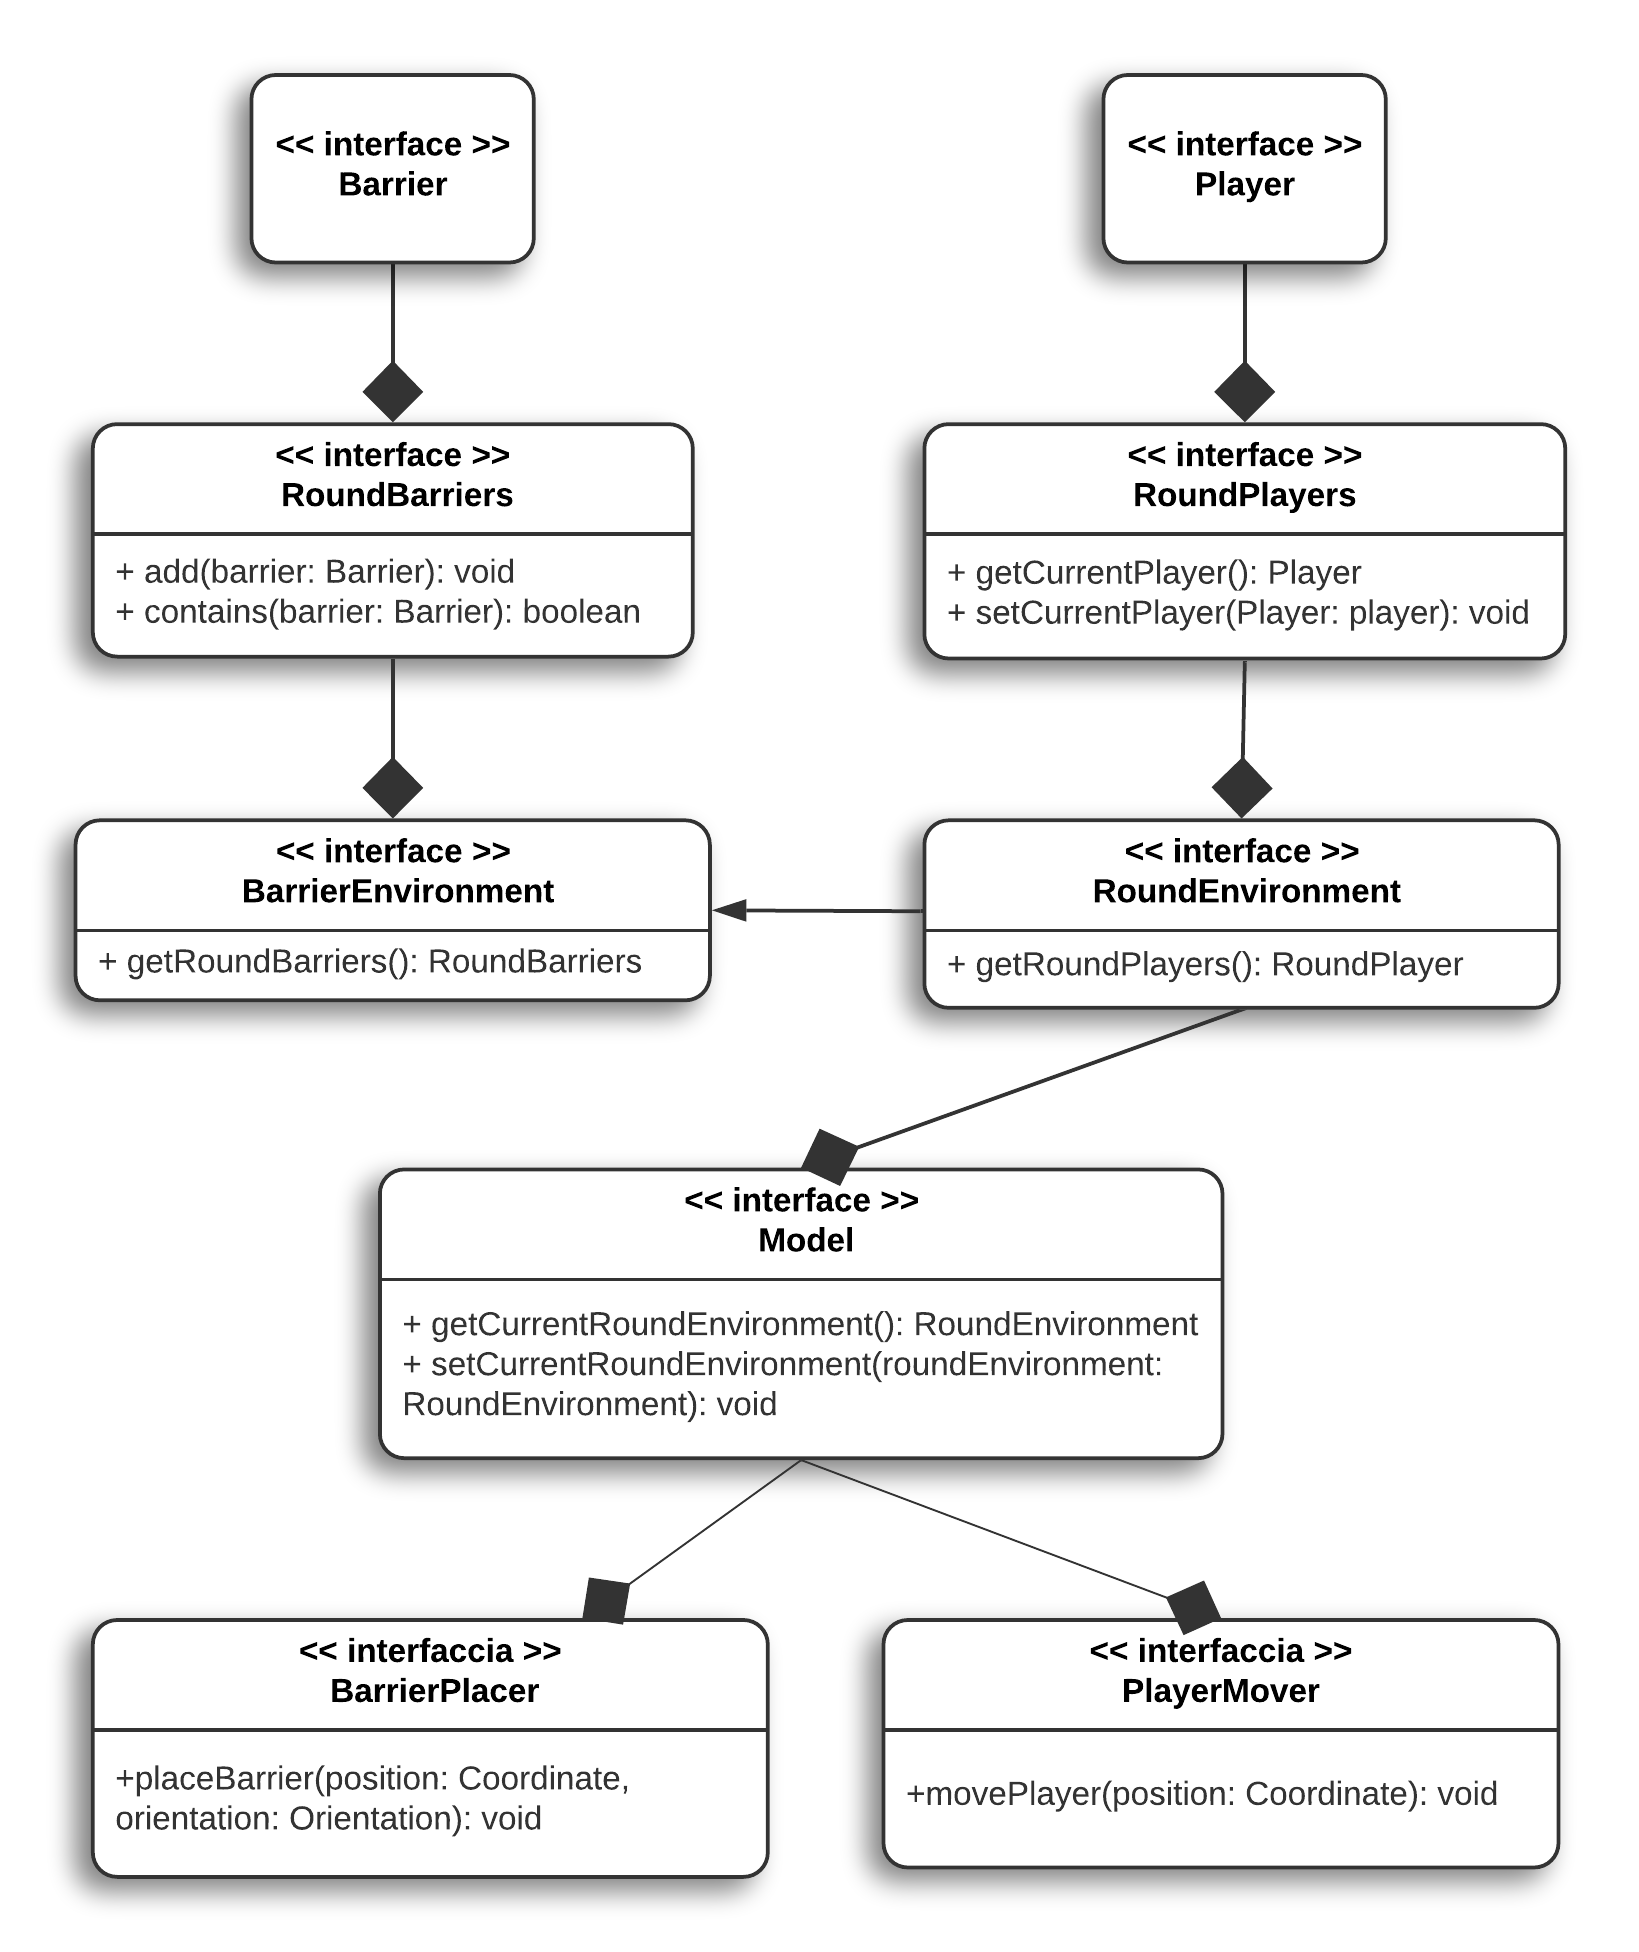
\includegraphics{modello_del_dominio}
	\centering	
	\caption{schema UML raffigurante la rappresentazione del problema attraverso le entità principali della partita standard}
	\label{img:dominio}
	\end{figure}


\end{document}



\end{document}